% ======================================================================
% col: 20

\chapter{Analisi dei risultati}
In questo capitolo verranno comparate le tre strategie usate e descritte in questa tesi.
Verranno presentate delle metriche su cui l'ottimizzazione lavora e altre di contorno sulla
qualità del percorso generato corredate da grafici e rappresentazioni grafiche del tracciato.
Sono state prese in considerazione due mappe: il circuito di Spa-Francorchamps in Belgio e il circuito di
Monza.

I dati usati in questo capitolo sono stati estrapolati solamente dai file di output dell'ottimizzazione
e analizzati con l'uso di Jupyter Notebook.
\begin{figure}[H]
	\begin{center}
	\begin{subfigure}[l]{0.45\textwidth}
		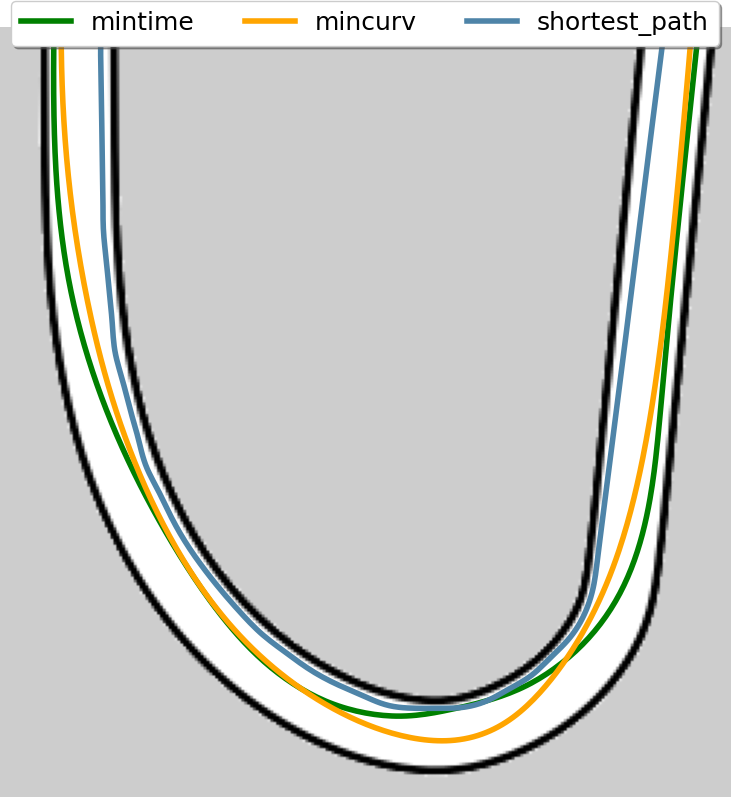
\includegraphics[width=\textwidth]{monza/raceline-parabolica.png}
	\end{subfigure}
	\begin{subfigure}[r]{0.5\textwidth}
		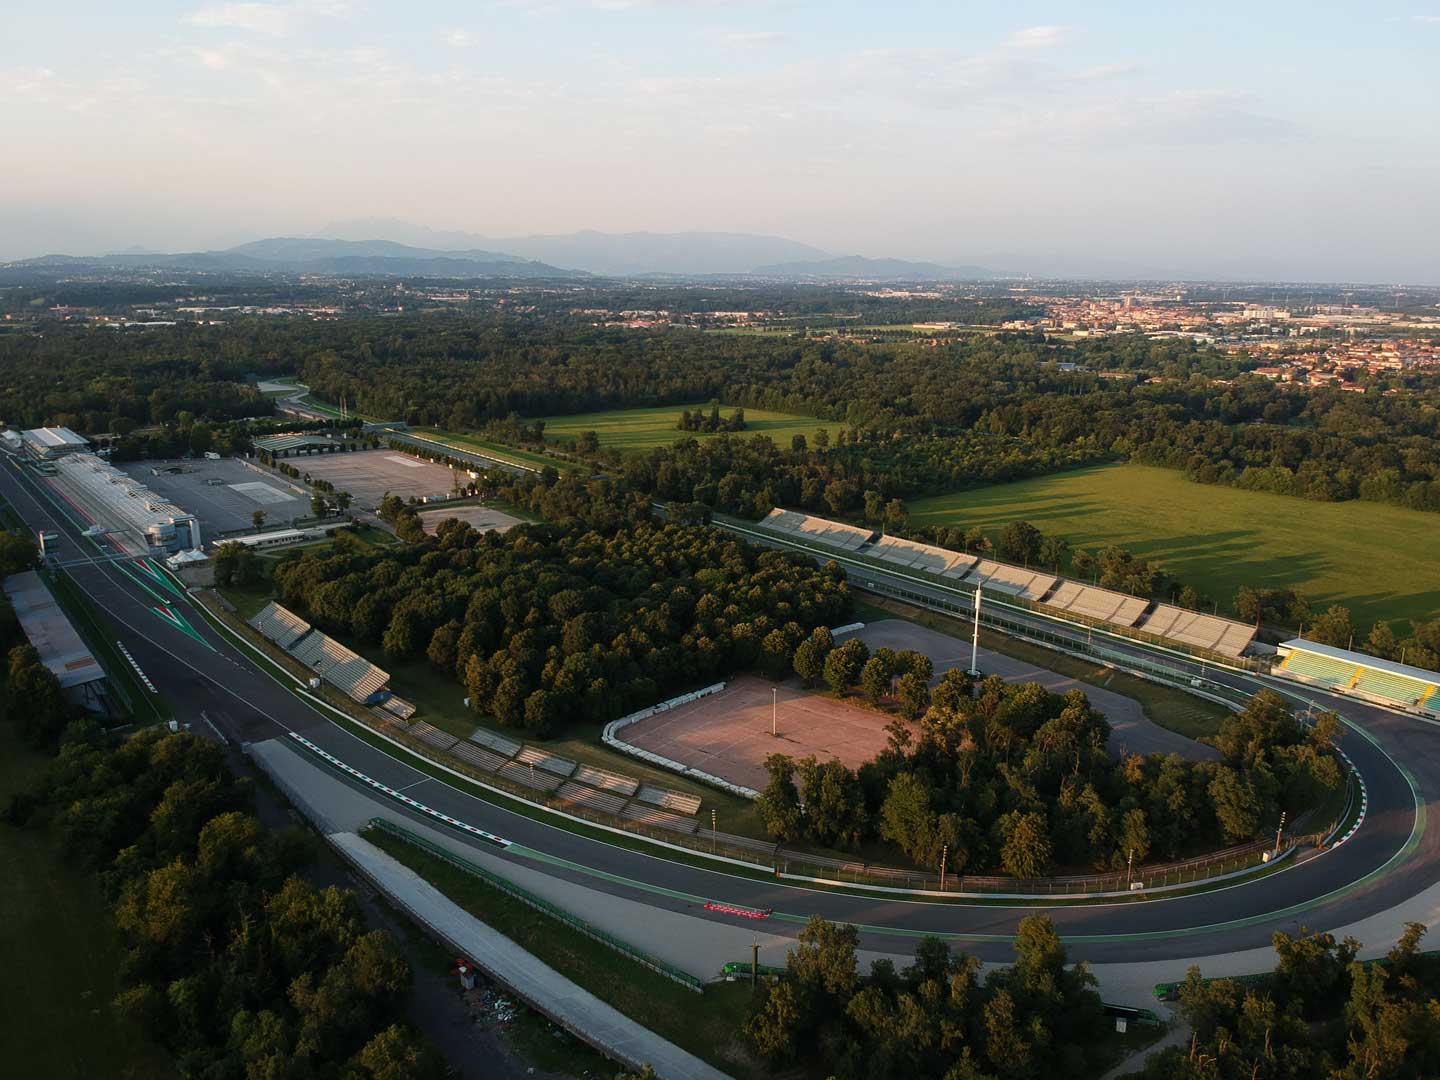
\includegraphics[width=\textwidth]{monza/curva-parabolica-foto-aerea.jpg}
	\end{subfigure}
	\end{center}
	% \caption{Raceline generate per la curva parabolica di Monza}
	% \label{fig:raceline-parabolica}
\end{figure}
\newpage
\section{Metriche}
Le metriche usate in questo studio sono le seguenti:
\begin{itemize}
	\item Il tempo di percorrenza (laptime);
	\item Lunghezza del tracciato prodotto;
	\item Velocità; %media, mediana, minima e la sua deviazione standard;
	\item Accelerazione; % mediana, massima e minima;
	\item Curvatura; %mediana e la sua deviazione standard;
	\item Tempo di esecuzione.
\end{itemize}
Le metriche scelte permettono di confrontare le tre strategie considerando quale criterio 
ottimizzano: il laptime per la strategia del percorso col tempo minimo, la lunghezza del tracciato per
quella del percorso più corto e, infine, la curvatura per la strategia della curvatura minima.
Ulteriori metriche di contesto sono la velocità, l'accelerazione e il tempo di esecuzione dei tre
algoritmi.

Per ogni mappa e per ogni strategia vengono confrontati laptime, curvatura mediana e la lunghezza del
tracciato risultante. Si è scelta la curvatura mediana perché quella media risultava sempre molto
vicino a zero e quindi poco significativa per effettuare un confronto. Egual discorso per
l'accelerazione, che tende a bilanciarsi tra accelerazioni e decelerazioni; a questa vengono anche
aggiunte la deviazione standard, l'accelerazione massima e minima. Viene poi indicata la velocità media,
la sua deviazione standard, la mediana e la minima, dato che la massima è stata impostata a $15\
\nicefrac{m}{s}$.

Di seguito si mostrano le misurazioni per i due circuiti di Monza e Spa.

% ================== SPA ===============================================
\section{Spa}
\label{sec:spa}
\begin{table}[H]
	\caption{Circuito di Spa}
	\label{tab:opt-spa}
	\begin{center}
		\begin{tabular} {l|c|c|c}
			                & Laptime [$s$]  & Curvatura mediana [$\nicefrac{rad}{m}$] & Lunghezza [$m$]\\
			\hline
			mintime         & \textit{76.25} & 0.10           & 545.41          \\
			mincurv         & 49.22          & \textit{0.07 } & 546.87          \\
			shortest path   & 55.12          & 0.09           & \textit{532.98} \\
			\hline
		\end{tabular}
	\end{center}
\end{table}
Per quanto riguarda la curvatura e la lunghezza del circuito, le strategie di mincurv e shortest path
effettivamente producono rispettivamente il risultato minore tra le strategie. Pare inaspettato il
risultato per il tempo minimo, che è il più alto tra tutte le strategie, questo tuttavia è giustificato
dalla migliore modellazione della dinamica del veicolo da parte dell'algoritmo: in questo senso, sebbene
mincurv e shortest path abbiano un laptime minore, questo è anche meno affidabile rispetto al mintime. Il
laptime viene calcolato sommando il tempo di percorrenza tra un sample e il successivo assumendo che la
velocità rimanga costante tra questi due: dunque un tracciato con una velocità media più alta risulterà
con un laptime minore; come si può notare dalla tabella~\ref{tab:spa-velocity}, la velocità media della
strategia mintime è decisamente inferiore rispetto alle altre due.

A conferma della più completa modellazione di mintime sono state le simulazioni con MPC sul
simulatore per le quali, a fronte del percorso di mincurv, il robot raggiungeva una velocità troppo
elevata e non riusciva a seguire bene il tracciato, uscendo spesso fuori dal circuito; mentre per quanto
riguarda il tracciato di mintime il controller riusciva a seguire meglio il percorso.

\begin{table}[H]
	\caption{Velocità in $\nicefrac{m}{s}$ per Spa}
	\label{tab:spa-velocity}
	\begin{center}
		\begin{tabular}{l|r|r|r|r}
			              & \thead{Media} & \thead{Mediana} & \thead{Minima} & \thead{Dev. std} \\
			\hline
			mintime       &  8.33 &  8.44 &  2.3 & 2.93 \\
			mincurv       & 12.05 & 12.82 & 3.47 & 2.88 \\
			shortest path & 10.79 & 11.29 & 1.63 & 2.97 \\
			\hline
		\end{tabular}
	\end{center}
\end{table}

\begin{figure}
	\begin{center}
	\begin{subfigure}[c]{0.3\textwidth}
		\includegraphics[width=\textwidth]{spa/mintime-velocity-prof.png}
		\caption{mintime}
	\end{subfigure}
	\begin{subfigure}[c]{0.3\textwidth}
		\includegraphics[width=\textwidth]{spa/mincurv-velocity-prof.png}
		\caption{mincurv}
	\end{subfigure}
	\begin{subfigure}[c]{0.365\textwidth}
		\includegraphics[width=\textwidth]{spa/shortest-velocity-prof.png}
		\caption{shortest path}
	\end{subfigure}
		\caption{Confronto della velocità per le tre strategie}
		\label{fig:spa-vel-comparison}
	\end{center}
\end{figure}

Come accennato al paragrafo precedente, la velocità media e mediana più alta appartiene alla strategia
della curvatura minima, il che rimane in linea con la formulazione del problema, ovvero mantenere la
velocità più alta in curva. Lo stesso è visivamente immediato osservando la figura~
\ref{fig:spa-vel-comparison}, dove mincurv tende ad avere colori più verso il verde nelle curve rispetto
alle altre due strategie.

La deviazione standard delle tre strategie rimane pressoché simile: solo il percorso più breve ne riporta
una più alta che è congrua anche con la variabilità dell'accelerazione nella tabella~\ref{tab:spa-ax}.

Come è possibile notare dal grafico~\ref{fig:speed-graph-spa}, solo mintime non ha mai toccato la massima
velocità impostata, raggiungendo un picco di $14.7\ \nicefrac{m}{s}$ e solo per pochissimo tempo, mentre
le altre due l'hanno tenuta per più tempo, mincurv tra tutte.
\begin{figure}[H]
	\begin{center}
		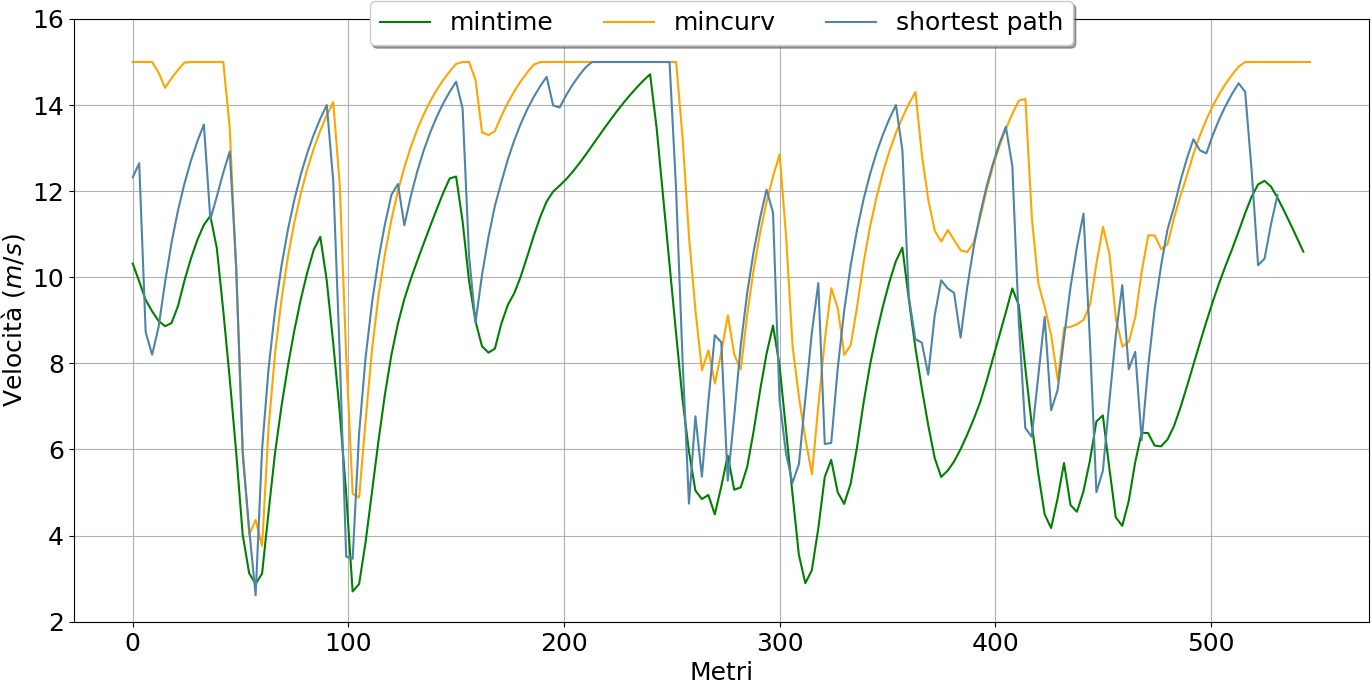
\includegraphics[width=\textwidth]{spa/speed-graph.png}
	\end{center}
	\caption{Profilo della velocità in Spa}
	\label{fig:speed-graph-spa}
\end{figure}
\begin{figure}[H]
	\begin{center}
		\includegraphics[width=\textwidth]{spa/acc-graph.png}
	\end{center}
	\caption{Profilo dell'accelerazione per Spa}
	\label{fig:acc-graph-spa}
\end{figure}
Nell'accelerazione si notano le maggiori differenze: si nota come la strategia del percorso minimo sia
molto aggressiva nel cambio di accelerazione, infatti ha la deviazione standard maggiore tra tutte. 
È da sottolineare che i valori di massimo e minimo sono spesso picchi che vengono mantenuti solo per
qualche frazione di metro -- come mostrato in figura~\ref{fig:acc-graph-spa} -- e quindi poco
significativi nell'insieme; per questo, oltre a quanto scritto precedentemente, si è scelto di usare la
mediana. In ogni caso, possono dare un'idea del dei valori assunti, e quindi indicare quanto estremo
è il range della strategia del percorso minimo rispetto al tempo minimo.

Qualitativamente, dall'immagine~\ref{fig:spa-acc-comparison}, si può notare come l'algoritmo per mintime
produca una serie di accelerazioni e decelerazioni più graduale rispetto alle altre due, soprattutto con
shortest path. Questo repentino e significativo cambio di accelerazione da parte di quest'ultimo, e di
mincurv in misura minore come mostra la figura~\ref{fig:acc-graph-spa}, produce dei tracciati difficili
da applicare nella realtà e quindi di
minor qualità rispetto a mintime.

\begin{table}[H]
\caption{Accelerazione in $\nicefrac{m}{s^2}$ per Spa}
\label{tab:spa-ax}
\begin{center}
	\begin{tabular}{l|r|r|r|r}
					  & \thead{Mediana} & \thead{Massima} & \thead{Minima} & \thead{Dev. std} \\
		\hline
		mintime       &  0.79 &  2.57 & -11.54 & 2.09 \\
		mincurv       &  0.75 &  4.98 & -15.29 & 3.05 \\
		shortest path &  1.83 &  5.29 & -16.27 & 5.11 \\
		\hline
		\end{tabular}
	\end{center}
\end{table}

\begin{figure}
	\begin{center}
	\begin{subfigure}[c]{0.3\textwidth}
		\includegraphics[width=\textwidth]{spa/mintime-acc-prof.png}
		\caption{mintime}
	\end{subfigure}
	\begin{subfigure}[c]{0.3\textwidth}
		\includegraphics[width=\textwidth]{spa/mincurv-acc-prof.png}
		\caption{mincurv}
	\end{subfigure}
	\begin{subfigure}[c]{0.383\textwidth}
		\includegraphics[width=\textwidth]{spa/shortest-acc-prof.png}
		\caption{shortest path}
	\end{subfigure}
		\caption{Confronto dell'accelerazione per le tre strategie}
		\label{fig:spa-acc-comparison}
	\end{center}
\end{figure}

% ================== MONZA =============================================
\section{Monza}
\begin{table}[H]
	\caption{Circuito di Monza}
	\label{tab:opt-monza}
	\begin{center}
		\begin{tabular} {l|c|c|c}
			                & Laptime [$s$]  & Curvatura mediana [$\nicefrac{rad}{m}$] & Lunghezza [$m$]\\
			\hline
			mintime         & \textit{50.72} & -0.07           & 441.37         \\
			mincurv         & 33.74          & \textit{-0.03 } & 439.57         \\
			shortest path   & 41.37          & -0.12           & \textit{434.1} \\
			\hline
		\end{tabular}
	\end{center}
\end{table}
Anche in questo caso valgono le stesse considerazioni descritte per il circuito di \href{sec:spa}{Spa} sopra
analizzato: gli algoritmi per mincurv e shortest path producono il risultato minore per le rispettive
metriche, mentre sono poco affidabili per il laptime, di cui mintime offre un risultato più realistico per
via della sua formulazione. Una nota da sottolineare è che l'algoritmo per mincurv è riuscito a
minimizzare maggiormente la curvatura rispetto alla mappa precedente; in questo senso minimizzare si
intende tendere a zero, dunque è necessario considerare i valori assoluti per la colonna della curvatura
alla tabella \ref{tab:opt-monza}.
\begin{table}[H]
	\caption{Velocità in $\nicefrac{m}{s}$ per Monza}
	\label{tab:vel-monza}
	\begin{center}
		\begin{tabular}{l|r|r|r|r}
			              & \thead{Media} & \thead{Mediana} & \thead{Minima} & \thead{Dev. std} \\
			\hline
			mintime       &  9.84 &  9.82 & 3.21 & 3.09 \\
			mincurv       & 13.41 & 14.56 & 7.88 & 2.04 \\
			shortest path & 11.34 & 11.52 & 4.67 & 2.83 \\
			\hline
		\end{tabular}
	\end{center}
\end{table}
\begin{figure}
	\begin{center}
	\begin{subfigure}[c]{0.3\textwidth}
		\includegraphics[width=\textwidth]{monza/mintime-velocity-prof.png}
		\caption{mintime}
	\end{subfigure}
	\begin{subfigure}[c]{0.3\textwidth}
		\includegraphics[width=\textwidth]{monza/mincurv-velocity-prof.png}
		\caption{mincurv}
	\end{subfigure}
	\begin{subfigure}[c]{0.365\textwidth}
		\includegraphics[width=\textwidth]{monza/shortest-velocity-prof.png}
		\caption{shortest path}
	\end{subfigure}
		\caption{Confronto della velocità per le tre strategie}
		\label{fig:monza-vel-comparison}
	\end{center}
\end{figure}
Anche per la velocità valgono alcune considerazioni fatte per Spa: la strategia di mintime è più
conservativa rispetto alle altre, ma in questo caso ha la deviazione standard più alta tra tutte.
In questo caso, anche mintime ha raggiunto la velocità massima indicata, tuttavia l'ha raggiunta solo una
volta e comunque per pochi metri, come è possibile alla figura \ref{fig:speed-graph-monza}; mentre,
anche in questo caso, mincurv è al primo posto per aver mantenuto per più tempo la velocità massima,
complice anche la topologia della mappa che offre maggiori possibilità grazie ai suoi rettilinei.
\begin{figure}[H]
	\begin{center}
		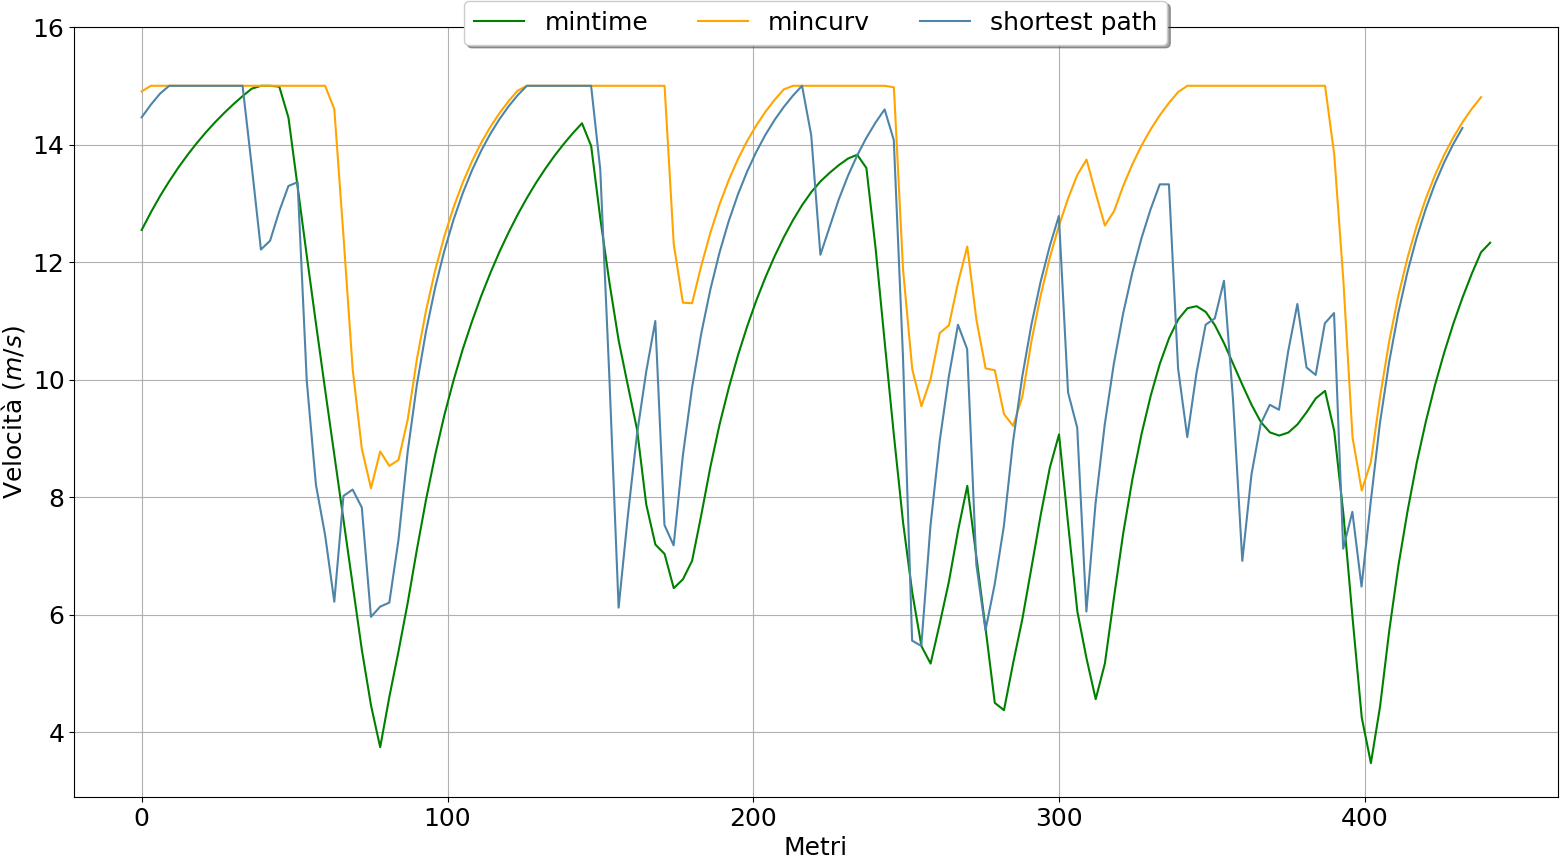
\includegraphics[width=\textwidth]{monza/vel-graph.png}
	\end{center}
	\caption{Profilo della velocità per Monza}
	\label{fig:speed-graph-monza}
\end{figure}
\begin{figure}[H]
	\begin{center}
		\includegraphics[width=\textwidth]{monza/acc-graph.png}
	\end{center}
	\caption{Profilo dell'accelerazione per Monza}
	\label{fig:acc-graph-monza}
\end{figure}
A differenza di Spa, la variabilità della strategia del percorso più breve risulta in linea con le altre
strategie e la sua mediana risulta simile alla rispettiva di Spa, come risulta dalla tabella
\ref{tab:acc-monza}. Spicca il valore fuori scala dell'accelerazione massima della strategia di mintime:
analizzando il dataset e osservando il grafico alla figura \ref{fig:acc-graph-monza} si nota
immediatamente che si tratta di un outlier generato, tra l'altro, solo per un singolo sample e quindi non
veramente applicabile dal robot reale o simulato. In ultima analisi, si tratta di un errore relativo a
questa esecuzione in particolare.

Qualitativamente dalla figura \ref{fig:monza-acc-comparison}, anche in questo circuito si nota come
mintime sia più graduale, soprattutto rispetto a shortest path, dove si può osservare molte volte
repentini sbalzi di accelerazione, che sono impraticabili per un veicolo.

\begin{table}[H]
	\caption{Accelerazione in $\nicefrac{m}{s^2}$ per Monza}
	\label{tab:acc-monza}
	\begin{center}
		\begin{tabular}{l|r|r|r|r}
			              & \thead{Mediana} & \thead{Massima} & \thead{Minima} & \thead{Dev. std} \\
			\hline
			mintime       &  0.80 & 17.98 &  -7.11 & 2.22 \\
			mincurv       &  0.00 &  4.00 & -15.48 & 2.86 \\
			shortest path &  1.63 &  4.78 & -16.31 & 3.13 \\
			\hline
		\end{tabular}
	\end{center}
\end{table}
\begin{figure}
	\begin{center}
	\begin{subfigure}[c]{0.3\textwidth}
		\includegraphics[width=\textwidth]{monza/mintime-acc-prof.png}
		\caption{mintime}
	\end{subfigure}
	\begin{subfigure}[c]{0.3\textwidth}
		\includegraphics[width=\textwidth]{monza/mincurv-acc-prof.png}
		\caption{mincurv}
	\end{subfigure}
	\begin{subfigure}[c]{0.383\textwidth}
		\includegraphics[width=\textwidth]{monza/shortest-acc-prof.png}
		\caption{shortest path}
	\end{subfigure}
		\caption{Confronto dell'accelerazione per le tre strategie}
		\label{fig:monza-acc-comparison}
	\end{center}
\end{figure}

% ================== Tempo di Esecuzione ===============================
\section{Tempo di Esecuzione} % NOTE: Tempo di Risoluzione
Un aspetto interessante che è stato analizzato è il tempo di esecuzione per ogni algoritmo. In generale
si è sperimentato un tempo tra pochi secondi e alcuni minuti dal lancio del solutore fino
all'esportazione in csv del risultato; tuttavia questo tempo racchiude anche controlli sul percorso
generato ed eventuali input dell'utente, quindi non è un buon indicatore del singolo processo di
risoluzione. Dunque si è fatto riferimento alla sola risoluzione del problema matematico e non a processi
precedenti o successivi.

Di seguito si mostra una tabella che indica il numero di secondi del tempo di risoluzione di ogni
strategia per 6 valori di \verb|stepsize_reg| diversi, mentre \verb|stepsize_prep| è stato fissato a
$0.75$ e \verb|stepsize_interp_after_opt| a 0.15.
\begin{table}[H]
	\caption{Tempo di esecuzione in $s$ per ogni stepsize}
	\label{tab:step}
	\begin{center}
		\begin{tabular}{l|r|r|r|r|r|r}
			Stepsize        & \thead{0.75} & \thead{1.00} & \thead{1.5} & \thead{2.0} & \thead{2.5} & \thead{3.0} \\
			\hline
			mintime       & fallito & fallito & 526.88 & 266.29 & 257.09 & 138.59 \\
			mincurv       & 0.798   & 0.372   & 0.167  &  0.094 &  0.072 &  0.048 \\
			shortest path & 0.361   & 0.313   & 0.086  &  0.041 &  0.022 &  0.013 \\
			\hline
		\end{tabular}
	\end{center}
\end{table}
Sono evidenti i fallimenti della strategia del percorso più breve a i primi due valori dello stepsize, la
motivazione è stata data al capitolo~\ref{chap:impl} al paragrafo~\ref{par:tuning}, pag.~
\pageref{par:tuning}. Si nota, in ogni caso, un'importante differenza di scala tra il tempo minimo e le
altre due strategie, questo è dato principalmente dalla complessità e una più completa modellazione del
veicolo dell'algoritmo e che quindi ha bisogno di una maggiore computazione, come descritto al capitolo~
\ref{chap:opt}, pag.~\pageref{chap:opt}.

Come anche accennato al paragrafo sopra citato, si può notare che l'aumentare degli stepsize spesso
dimezzi la velocità nel trovare una soluzione, o in generale la diminuisce, dato appunto dal numero minore
di sample da considerare.
In figura~\ref{fig:stepsize_fviz} si può osservare come l'andamento di tutte le tre strategie possa
essere approssimato grossomodo ad una funziona quadratica inversa.
\begin{figure}[H]
	\begin{center}
		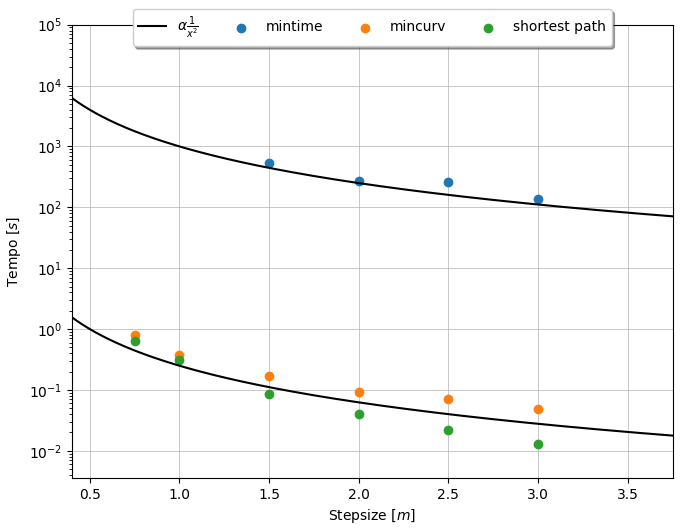
\includegraphics[width=0.9\textwidth]{stepsize_func_viz.png}
	\end{center}
	\caption{Grafico dell'andamento del tempo di esecuzione secondo diversi valori di
	\texttt{stepsize\_reg}}
	\label{fig:stepsize_fviz}
\end{figure}

